\chapter{Discussion and Conclusion}\label{cha:discussion-and-conclusion}

\begin{comment}
When evaluating your results, avoid drawing grand conclusions, beyond those that your results can in fact support.
Further, although you may have designed your experiments to answer certain questions,
the results may raise other questions in the eyes of the reader.
It is important that you study the graphs/tables to look for unusual features/entries, and discuss these as well as the main findings.
In particular, carry out an error analysis: What went wrong and why?

A confusion matrix can, for example, be a good way to display misclassifications.
Figure~\ref{fig:conf_sentiment} (on Page~\pageref{fig:conf_sentiment}) shows two confusion matrices.
If there were perfect correlation between true and predicted labels, the long diagonals (from the upper left to the lower right corner) would be completely red.
However,  the confusion matrices indicate
that this classifier was quite biased towards the neutral label (illustrated with \Neutrey),
as can be seen from the warm colours in the positive (\Smiley) and negative (\Sadey) true label cells of the \Neutrey predicted label column.

% Axis configuration for confusion matrices with pgfplots
\pgfplotsset{
    colormap={whitehot}{color(0cm)=(white); color(1cm)=(yellow); color(2cm)=(orange); color(3cm)=(red)},
    confusionaxis/.style={
            colorbar,
            colorbar style={
                    width=2mm,
                    at={(1.05,1)},
                },
            colormap name=whitehot,
            faceted color=none, % remove lines between fields
            view={0}{90},
            y dir=reverse,
            xlabel=Predicted label,
            ylabel=True label,
            tick style={draw=none},
            yticklabels={,,},
            xticklabels={,,},
            every node=[font=\small],
            extra x ticks={0.4,1.5,2.6},
            extra x tick labels={\Smiley, \Neutrey, \Sadey},
            extra y ticks={0.3,1.5,2.7},
            extra y tick labels={\Smiley, \Neutrey, \Sadey},
            extra x tick style={
                    x tick label style={
                            font=\Large
                        }
                },
            extra y tick style={
                    y tick label style={
                            font=\Large
                        }
                },
            width=.4\linewidth,
        }
}

\begin{figure}[t!]
    \centering
    \begin{subfigure}{\linewidth}
        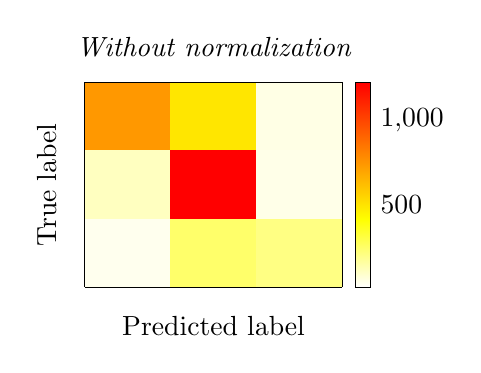
\begin{tikzpicture}
            \begin{axis}[
                    confusionaxis,
                    title={\em Without normalization},
                ]
                \addplot3
                [surf,mesh/cols=4,shader=flat corner
                ] coordinates {
                        (0,0,740) (1,0,490 ) (2,0,43 ) (3,0,1)
                        (0,1,102) (1,1,1229) (2,1,38 ) (3,1,1)
                        (0,2,28 ) (1,2,240 ) (2,2,199) (3,2,1)
                        (0,3,1  ) (1,3,1   ) (2,3,1  ) (3,3,1)
                    };
            \end{axis}
        \end{tikzpicture}
        %\hfill
        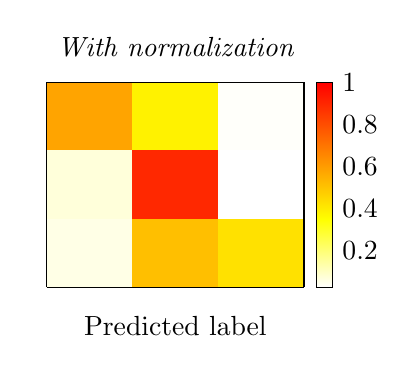
\begin{tikzpicture}
            \begin{axis}[
                    confusionaxis,
                    title={\em With normalization},
                    ylabel={},
                    colorbar style={
                            ylabel={},
                            yticklabel style={
                                    align=right,
                                }
                        },
                ]
                \addplot3
                [surf,mesh/cols=4,shader=flat corner
                ] coordinates {
                        (0,0,0.58130401) (1,0,0.38491752) (2,0,0.03377848) (3,0,1)
                        (0,1,0.07450694) (1,1,0.89773557) (2,1,0.02775749) (3,1,1)
                        (0,2,0.05995717) (1,2,0.51391863) (2,2,0.4261242 ) (3,2,1)
                        (0,3,1         ) (1,3,1         ) (2,3,1         ) (3,3,1)
                    };
            \end{axis}
        \end{tikzpicture}
        \label{fig:conf_sentiment_2013}
    \end{subfigure}
    \caption{Sentiment classifier confusion matrices}
    \label{fig:conf_sentiment}
\end{figure}
\end{comment}

\begin{comment}
In this section it is important to include a discussion of not just the merits of the work conducted, but also the limitations.
Which choices did you make? Why? What alternatives were there?
{\color{red}\textbf{Note that a key part of the Master's Thesis grading is based on the student's ability to discuss the results in light of the work by others as well as the restrictions and potential of the work itself.}}
While the Results section will report the outcome of each specific experiments, the Discussion should put those results into perspective and look at overall lessons that can be learned from the entire series of experiments.

You should be able to discuss your work in relation to its overall goal and your research questions (i.e., those introduced in Chapter~\ref{cha:introduction}),
but also address issues such as any ethical considerations that the work may entail,
as well as its technical challenges and limitations.

Discussion and evaluation can either be two different chapters, a joint chapter (as here), or part of the concluding chapter
--- or the discussion can be part of that chapter while the evaluation is part of the experimental chapter.

As for most parts of the thesis, it is possible to select various outlines and setups for the discussion; the important thing is that all the relevant parts appear \textit{somewhere\/} in the text.
\end{comment}

% \cite{yiuTransmissionTruthImitation2023} calls \acrshort{acr:ai} technologies like \acrlongpl{acr:llm} "powerful imitation engines" but claim that they are unable to innovate and that significant advancements in \acrshort{acr:ai} development is required for them to be able to learn the in the same way human children do.

Sections \autoref{sec:code-interpreter-discussion} and \autoref{sec:api-access-discussion} will discuss the experimental results (see \autoref{sec:experimental-results}), and providing suggestions as to how the limitations highlighted by the experiments can be mitigated. \Autosectionref{sec:conclusion-and-future-work} will conclude this specialization project report, and provide directives for future work on the subject of \acrshort{acr:llm}-power \acrshort{acr:gis}.

\section{Using the In-Built ChatGPT Code Interpreter for Geospatial Analysis}\label{sec:code-interpreter-discussion}

When using ChatGPT's Code Interpreter with file uploads, it became apparent that it runs in a Linux environment, and that it uses a mounted drive  in the \texttt{/mnt} director, which is used for temporarily mounted filesystems. From the initial experiments where the same data in different file formats was tested it tried to a \acrshort{acr:gdal} command (\texttt{ogr2ogr -f "GeoJSON" \{converted\_geojson\_path\} \{sosi\_file\_path\}}) to perform a conversion from \acrshort{acr:sosi} to GeoJSON, the latter of which is far easier to manipulate in a Python environment. This test failed, and the system's response was that \enquote{the \texttt{ogr2ogr} tool is not available in this environment}.

This result was not very surprising, especially since the driver needed to read and write \acrshort{acr:sosi} files---which is called \textit{fyba} and is developed by The Norwegian Mapping Authority\footnote{\url{https://github.com/kartverket/fyba}}---is almost certaintly not available in the standard Linux environment for ChatGPT's Code Interpreter. Seeing as the \acrshort{acr:sosi} standard still is widely used for Norwegian geospatial purposes (though expected to be exchanged with the \acrshort{acr:gml} format in the future), it is important for an \acrshort{acr:llm}-based \acrshort{acr:gis} agent focused on the Norwegian market to be able to handle this file type.

The inability to manipulate the Linux environment using by the Code Interpreter clearly poses some limitations on the systems. A solution to the problem is to create a custom environment on a server and implement agent-like capabilities by other means (LangChain, AutoGPT, AutoGen, etc.). Having the agent run on an environment that we control ourselves gives us greater flexibility, and we can then allow the agent to access powerful \acrshort{acr:gis} tooling, such as the \acrshort{acr:gdal} library. This also allows us to avoid having to perform I/O on a mounted directory (in the \texttt{/mnt} directory), which can increase the speed of reads and writes.

\section[Mitigating ChatGPT's Inability to Access Web APIs]{Mitigating ChatGPT's Inability to Access Web \acrshort{acr:api}s}\label{sec:api-access-discussion}

As results of experiment 2 (see \autoref{subsec:experiment-2-results}) showed, ChatGPT-4 struggles when provided with URLs to external Web APIs, even when prompted to use its web browsing abilities and pairing them with its Code Interpreter. These issues are not present when using direct file upload, in which case the model appears to save the uploaded file in a temporary file directory in on a mounted drive in its Linux environment. While it can be hard to interpret the inner workings only from the code samples, it appears that it does not do this by default after fetching data from an external \acrshort{acr:api}. It appears from the results, in which it \textit{truncates} the file and \enquote{store's} the content directly in code, thus attempting to store the entire file in the context window of the  \acrshort{acr:llm}. The context window of the ChatGPT-4 model is currently at 32,000 tokens (the new GPT-4 Turbo has a context length of 128,000 tokens). While these are of significant size, they are not meant to (or able to) store large file, and thus it becomes a limiting factor when the file contents grow large, which is not uncommon for geospatial files.

This is a significant limitation of using ChatGPT-4 out of the box, and one should therefore look into other ways of handling web requests and subsequent storing of the received data. Techniques within \gls{acr:rag} can help here, and tools like LangChain or OpenAI's own \enquote{GPTs}\footnote{\url{https://openai.com/blog/introducing-gpts}} can help solve this issue.

\section{Conclusion and Future Work}\label{sec:conclusion-and-future-work}

\begin{comment}
What are the main contributions made to the field?
How significant are these contributions?
Also discuss the contributions in terms of the goals and research questions formulated in the Introduction.

The contributions section will normally contain everything that you address in the abstract, but in an extended form and quite possibly additional issues that cannot be included in the abstract.
An obvious difference is that when the reader has come this far in the text, she/he should be quite familiar with the work, but while reading the abstract they will have little to no knowledge of the work.

The section ``Contributions'' in Chapter~\ref{cha:introduction} differs from this one in that the former is just a list of the main bits, while this section should explain them in more detail.
However, basically the same items should appear in both sections.

\section{Future Work}
\label{sec:futureWork}

Consider where you would like to extend or improve this work, or how somebody else could continue it.
These extensions might either be continuing the ongoing direction or taking a side direction that became obvious during the work.
Further, possible solutions to limitations in the work conducted, highlighted in Section~\ref{sec:discussion} may be presented.

Note that in the Specialisation Project Report, the Future Work section will be a key part of your plan for the novel work to be carried out in the next semester,
while in the Master's Thesis, the Future Work section rather will point to issues that others might be interested in addressing.
This can include options and alternatives that you did not try out yourself, or potential improvements and extensions to your experiments or system.
\end{comment}

This specialization project has displayed an extensive literature research in the fields of \acrlong{acr:nlp}, \acrlongpl{acr:llm}, and \acrlong{acr:gis}, along with two experiments trying to learn display strengths and limitations of \acrshortpl{acr:llm} when dealing with geospatial data in different file formats. The literature and experiments serve as a preliminary study to provide a better starting point when attempting to develop an \acrshort{acr:llm}-based \acrshort{acr:gis} agent.

With this being a specialization project that will transition into a larger master thesis, some points of discussion have been reserved for future work. Additionally, the task of developing a proof of concept has been assigned to the master thesis due to time constraints and the intention to acquire more knowledge before proceeding with development. The following sections will elaborate on potentially important issues that needs to be addressed when developing an \acrshort{acr:llm}-based \acrshort{acr:gis} agent.

\subsection{Balancing Accuracy Against Performance and Costs}

The ecosystem of agent frameworks and planning strategies to improve agent performance on complex tasks (discussed in \nameref{cha:related-work}), is a growing one. Different agents frameworks and planning strategies should be compared to see which are most viable for \acrshort{acr:gis} work. Important considerations are the ability to destructure complex problems, the ability to take advantage of external tooling, and computational time. More complex planning strategies typically demand more interactions with \acrshort{acr:llm} \acrshortpl{acr:api}, which can be expensive both in terms of computational time and cost (when using a monetized \acrshort{acr:api} like OpenAI's for \acrshort{acr:gpt}-4 and \acrshort{acr:gpt}-4).

\cite{clearyLatencyBenchmarksComparisons2023} did benchmarking of different \acrshortpl{acr:llm} on different providers. Important takeaways were that \acrshort{acr:gpt}-4 is about 6.3 times slower than \acrshort{acr:gpt}-3.5-Instruct, and that Azure has far lower latency in most cases for inference on \acrshort{acr:gpt} models. Such considerations are important when addressing usability of \acrshort{acr:llm}-based applications, balancing accuracy against speed and costs. Using free open-source alternatives where possible is a good option to reduce costs.

\subsection{Testing regime}

In order to test the feasibility of different language models to serve as the brain of an autonomous \acrshort{acr:gis} agent, a testing regime should be developed. In the examples of autonomous \acrshort{acr:gis} agents described in the literature study of this report (see \autoref{sec:gis-with-llms}), results have generally been presented in the form of case studies \citep{liAutonomousGISNextgeneration2023,zhangGeoGPTUnderstandingProcessing2023}. This type of qualitative testing is entirely appropriate to showcase the possibilities of the technologies but may be insufficient when comparing performance of different systems. In the latter case a quantitative approach would probably be preferable.

One idea is to create a test dataset which consists of inputs and corresponding desired outputs of typical \acrshort{acr:gis} tasks. Inputs would in this case be natural language queries inputted by a mock user, and the output would be what you would expect a \acrshort{acr:gis} professional to return when given the same tasks/queries. Inputs should reflect the varying level of \acrshort{acr:gis} knowledge in the different user groups (see \autoref{sec:user-groups}). Outputs could be files with typical geospatial extensions (.shp, .geojson, .sosi, etc.), or they could adhere to API schemas specified by geospatial standards (see \autoref{sec:geospatial-standards}).

While the inputs should be fairly simple to construct there are several questions to be answered in regard to the outputs:

\begin{itemize}
    \item How does one evaluate the accuracy of the output?
    \item How should the \acrshort{acr:ai} agent respond when the user does not specify an output file format?
    \item How does one evaluate the usefulness of outputs to questions that should not return geospatial files, e.g. answers to general questions about geo-related subjects?
\end{itemize}

These are questions outside the scope of this specialization project. They will, however, be pursued in my master thesis.

\subsection{Memory and Embeddings}

Storing information for future use is important when developing \acrshort{acr:llm}-based agents in order for it to produce consistent responses. \cite{wengLLMPoweredAutonomous2023} three different types of memory in human brains: (1) \textit{Sensory Memory}, (2) \textit{Short-Term Memory}, and (3) \textit{Long-Term Memory}. When translated to \acrshort{acr:llm} we can think of \textit{Sensory Memory} as learning embedding representation, \textit{Short-Term Memory} as the memory contained within the limits of the context window of the Transformer, and  \textit{Long-Term Memory} as an external vector store that can be attended to by the agent at query time. Such a vector store/database would store the vector embeddings of the data contained within it, and allows for fast and accurate similarity search and retrieval based on the vector distance or similarity between the vector representations \citep{evchakiVectorDatabase2023}. \cite{wengLLMPoweredAutonomous2023} lists some common approximate nearest neighbours algorithms for fast retrieval speeds, including \gls{acr:lsh} and \gls{acr:faiss}.

Future work should expand on the work of \cite{unluChatmapLargeLanguage2023} (see \autoref{sec:gis-with-llms}) and investigate if vector embeddings can be used for long-term storage of geographical data with textual description, or if a vector database can be used to efficiently retrieve relevant resources like \acrshortpl{acr:api} or other external tools based on their documentation/specification. Additionally, this documentation and the \acrshort{acr:api} specifications can be large is size, and the context length can become a limiting issue. Vector embeddings can help mitigate such issues. By splitting the documents into chunks and indexing them using vector embeddings, one can extract only the relevant parts and pass these to the \acrshort{acr:llm} with the prompt.

\glsaddall